%----------------------------------------------------------------------------------------
%	PACKAGES AND OTHER DOCUMENT CONFIGURATIONS
%----------------------------------------------------------------------------------------

\documentclass{article} % Paper and 12pt font size
\usepackage[utf8]{inputenc}
\usepackage[T1]{fontenc}
% \usepackage{libertine}
\usepackage{lmodern} % Use font Latin Modern Sans Typewriter
% \renewcommand{\familydefault}{\ttdefault}
\usepackage[a4paper, margin=1in]{geometry} % Paper size and margin

\usepackage{enumitem} % Format the enumerated list
\usepackage{amsmath,amsfonts,mathtools} % Math packages
\usepackage{amsthm}
\interdisplaylinepenalty=2500
\usepackage{amssymb}
\usepackage[makeroom]{cancel}
\setlength\parindent{0pt} % Removes all indentation from paragraphs - comment this line for an assignment with lots of text

\usepackage{array}
\usepackage{tabu} % Table to text width
\renewcommand{\arraystretch}{1.} % The height of each row in the table is set to 1.5 relative to its default height.
\usepackage[table]{xcolor}

\usepackage{tikz} % Remember picture
\usepackage{graphicx} % Includes images
\graphicspath{ {./images/} } % Tells LATEX that the images are kept in a folder named images under the directory of the main document
\usepackage{wrapfig} % Wrap image i
\usepackage{eso-pic} % used for image background on titlepage


% Code listing style --------------
\usepackage{listings} % Code listing
\usepackage{color}
\definecolor{codegreen}{rgb}{0,0.6,0}
\definecolor{codegray}{rgb}{0.5,0.5,0.5}
\definecolor{codepurple}{rgb}{0.58,0,0.82}
\definecolor{backcolour}{rgb}{0.95,0.95,0.92}
\lstdefinestyle{mystyle}{
    backgroundcolor=\color{backcolour},
    commentstyle=\color{codegreen},
    basicstyle=\ttfamily\small,
    keywordstyle=\color{magenta},
    numberstyle=\tiny\color{codegray},
    stringstyle=\color{codepurple},
    breakatwhitespace=false,
    breaklines=true,
    captionpos=b,
    keepspaces=true,
    numbers=left,
    numbersep=5pt,
    showspaces=false,
    showstringspaces=false,
    showtabs=false,
    tabsize=2
}
\lstset{style=mystyle}
\usepackage{todonotes}  % Todo



%----------------------------------------------------------------------------------------
%	TITLE SECTION
%----------------------------------------------------------------------------------------
\title{\Huge \textbf{ASSIGNMENT 1} \vspace{.4in} \hrule}

\author{
	\Large ROB521: Mobile Robotics and Perception\\
	\Large Jojo (Yizhi) Zhou, 1003002396\\
}
\date{\normalsize\today}

\linespread{1.3}

\begin{document}
\fontfamily{lmtt} % modern typewriter font

%----------------------------------------------------------------------------------------
%	FRONT MATTER
%----------------------------------------------------------------------------------------
\begin{titlepage}
\tikz[remember picture,overlay]
\node[opacity=1] at (current page.center){
\includegraphics[width=\paperwidth,height=\paperheight]{../Background}};
\vspace*{3.5cm}
{\let\newpage\relax\maketitle}
\vspace*{\fill}

\end{titlepage}

% \newpage
\fontfamily{lmtt} % modern typewriter font

%----------------------------------------------------------------------------------------
%	Q1
%----------------------------------------------------------------------------------------
\section{Noise-free Wheel Odometry} % The * makes it an unnumbered section
\begin{figure}[hbt]
  \centering
    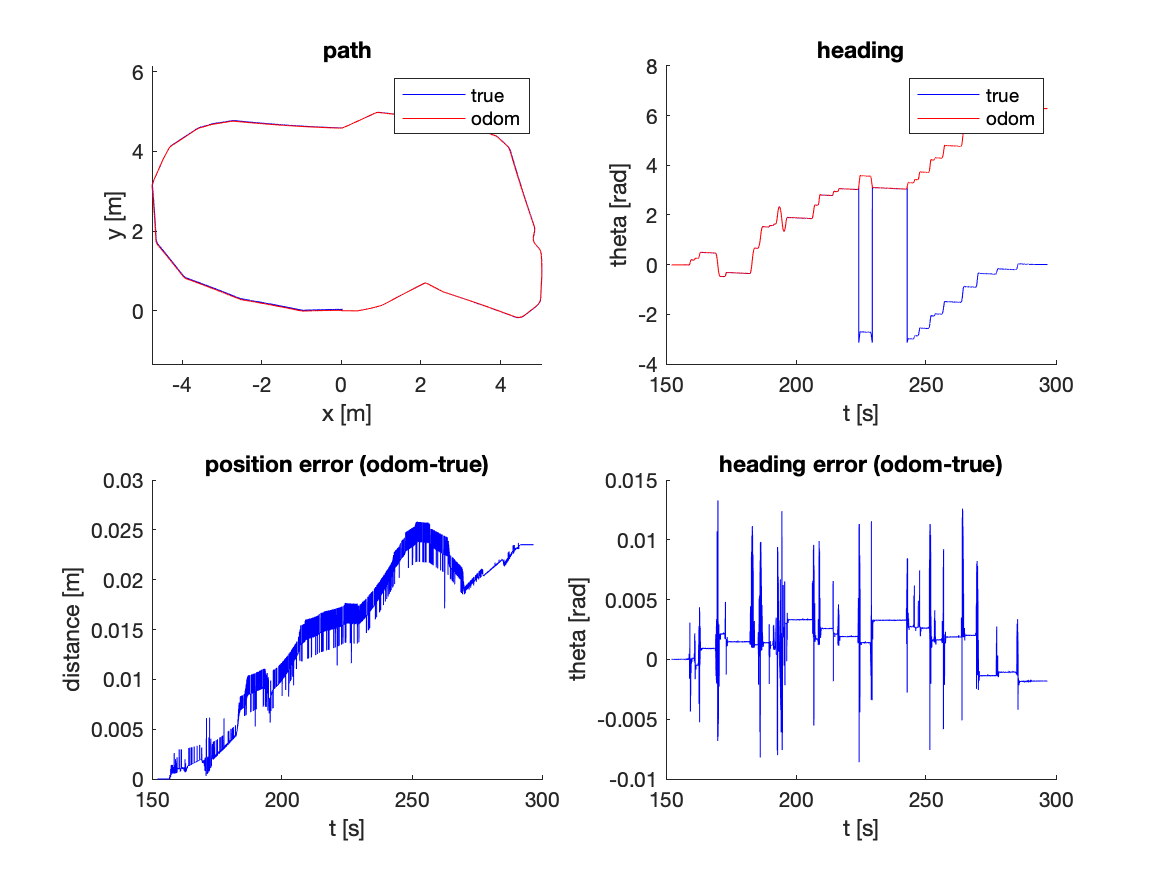
\includegraphics[width=1.0\textwidth]{ass1_q1.png}
  \caption{Output plot from to Question 1}
\end{figure}

The algorithm estimates the pose of robot using wheel odometry data, which is considered \textbf{noise-free} (i.e., no slipping and no measurement precision error in the encoder) in this part. 
\begin{itemize}
    \item \textbf{Position.} From the path plot, the ground truth and odometry are nearly identical. The position error ranging from 0 in the beginning to about 2.6 cm at worst and grows (roughly) proportionally. That being said, the error in centimeters is negligible compared to our scale of position in meters.

    \item \textbf{Heading.} The heading is quite accurate in the beginning as well, until around 230 seconds where there is a small period of offset. The same offset (i.e., $\sim2\pi$) occurred after 250 as well. Since the offset is essentially a full round, the offset is unlikely to be caused by an error; instead, it is likely due to the way that ROS/Gazebo/Turtlebot is designed, which seems to favor smaller angle changes (i.e., increment by $\delta\theta$ instead of $\delta\theta-2\pi$ if $|\delta\theta|<|\delta\theta-2\pi|$). However, none of such offset (or any offset of an integer number of full circles) would have an impact when we determine the pose of robot, as $\theta$ and $\theta\pm2\pi$ are practically equal to each other.
    
    From the error plot, we can see that the $2\pi$ offset was indeed not taken into account. Instead, we get a bunch of small errors. Through comparison with the heading plot, we can see that these small errors occur at sudden direction changes - the larger the increment/decrement in heading, the larger the error. This totally makes sense as the robot might needs to overshoot a little bit, physically, when as it changes its heading.
\end{itemize}

%----------------------------------------------------------------------------------------
%	Q2
%----------------------------------------------------------------------------------------
\section{Noisy Wheel Odometry} 
\begin{figure}[hbt]
  \centering
    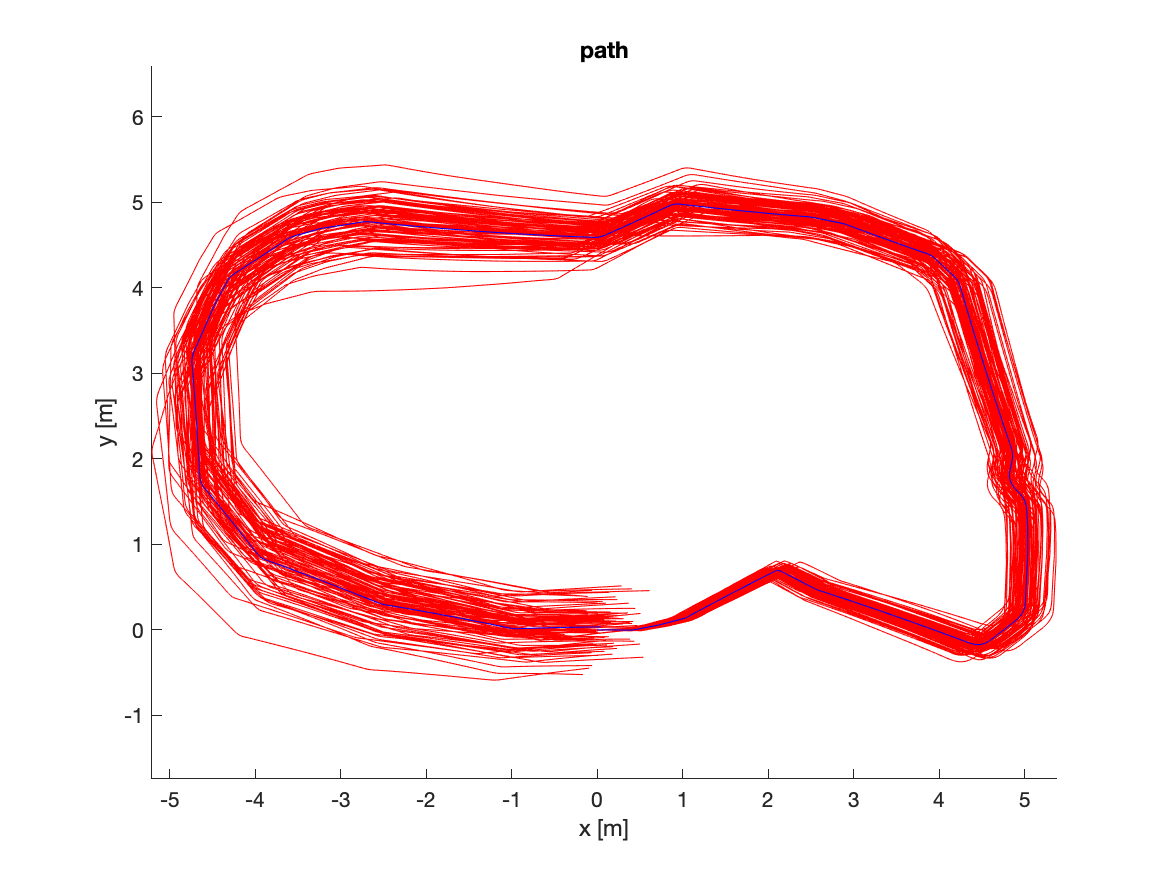
\includegraphics[width=0.9\textwidth]{ass1_q2.png}
  \caption{Output plot from to Question 2}
\end{figure}

The algorithm in this part remains the same as that in the previous part, with an addition of noise that simulates the real wheel odometry. We randomly sample 100 instances with from such noise and plot the 100 resulting paths in Figure 2. A few observations are worth being discussed:
\begin{itemize}
    \item Obviously, the paths starts at the same point as the ground truth and continues to diverge away from it, while the general trend still follows the ground truth.
    \item Mathematically speaking, as \texttt{randn} retunes scalars drawn from the standard \textit{normal distribution}, the random instances we generated have the noise-free velocities (i.e., same as ground truth) as mean values. Therefore, the expected path should indeed match the ground truth one, while the \textbf{error propagates}.
    \item Unlike part 1, this the result produced in this part doens't exactly match the reference solution, which makes sense since the samples are drawn randomly.
\end{itemize}

%----------------------------------------------------------------------------------------
%	Q3
%----------------------------------------------------------------------------------------
\section{Map from  Odometry} % The * makes it an unnumbered section
\begin{figure}[hbt]
  \centering
    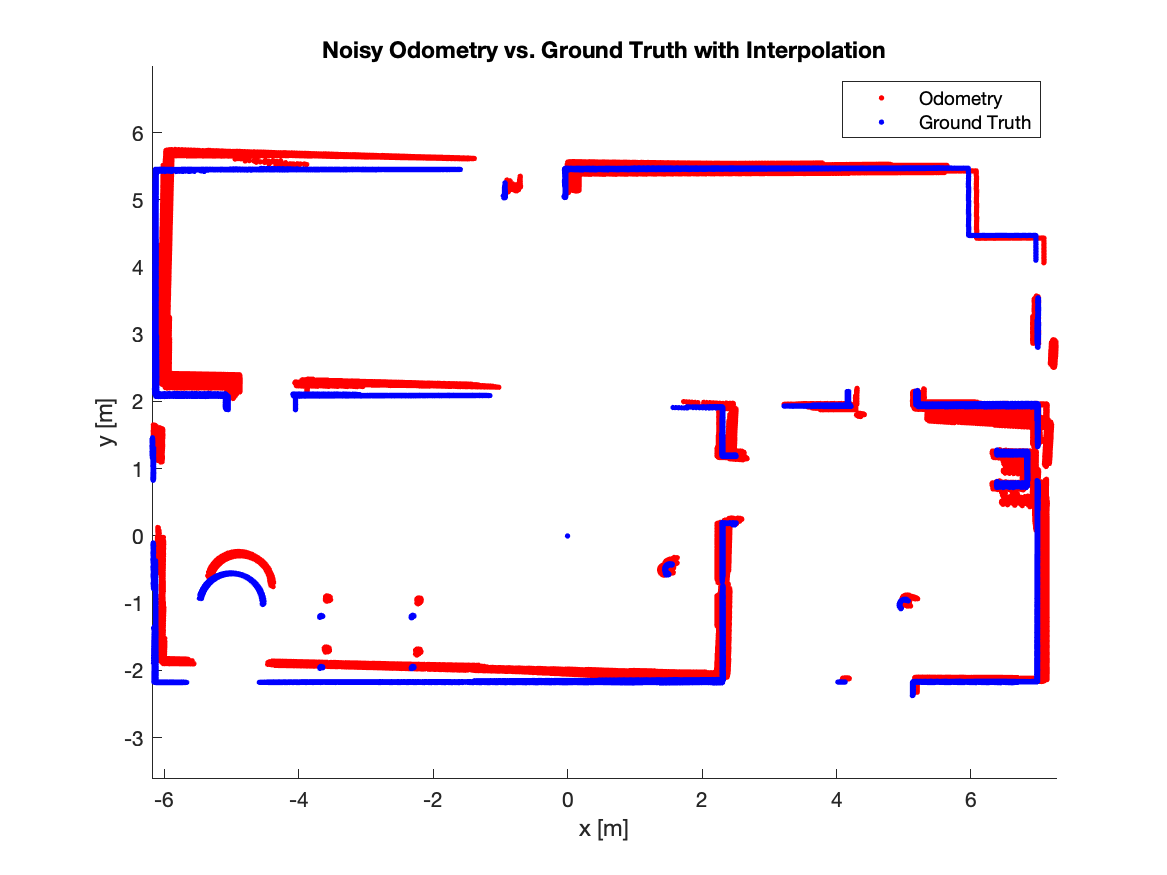
\includegraphics[width=0.9\textwidth]{ass1_q3.png}
  \caption{Output plot from to Question 3}
\end{figure}

For the noisy odometry data, the laser data gets more uncertain the longer the robot travels. This is expected as the odometry is a form of dead reckoning so the variance/uncertainty grows without bound. We can see growing errors in both the mean, as the odometry data is offset from the ground truth and sometime duplicated, and the variance, as the odometry landmarks are significantly thicker which indicates higher uncertainty.
While the two patches for angular velocity and laser position offset was applied, the resulting solution is still not as crisp as the sample solution. This does not appear to be simply a plotting error as the top-left corner is doubled in both plots, indicating some pose estimation errors in my algorithm.


%----------------------------------------------------------------------------------------
%	Appendix
%----------------------------------------------------------------------------------------
\clearpage
\section*{Appendix: Source Code}
\lstinputlisting[language=matlab]{ass1.m}


\end{document}
